\documentclass[11pt]{article}
\usepackage{amsmath}
\usepackage{amssymb}
\usepackage{geometry}
\usepackage{listings}
\usepackage{enumitem}
\usepackage{graphicx}

\usepackage{fancyhdr}
\pagestyle{fancy}
\fancyhf{}

\cfoot{\quad \quad \quad \quad \quad Lazuli \thepage}


\renewcommand{\headrulewidth}{0pt}
\geometry{margin=1in}

% Configuration for SAS code block formatting
\lstset{
    basicstyle=\ttfamily\small,
    breaklines=true,
    xleftmargin=2em
}

\begin{document}

\begin{center}
    {\LARGE \textbf{STAT 505 Assignment Submission [L5]}} \\  Ada Lazuli
\end{center}
\vspace{0.5em}

\begin{enumerate}
    \item \textit{(adapted from J\&W Exercise 1.6)} Various measurements on air pollution in Los Angeles are recorded in the data set ``air.csv''. Variables are $X_1 = \text{wind}$, $X_2 = \text{solar radiation}$, $X_3 = \text{CO}$, $X_4 = \text{NO}$, $X_5 = \text{NO}_2$, $X_6 = \text{O}_3$, and $X_7 = \text{HC}$.
    
    \begin{verbatim}
    data air;
    infile "/air.csv" delimiter="," firstobs=2;
    input x1-x7;
    run;
    \end{verbatim}
    
    \begin{enumerate}
        \item Explain briefly what $X_{ij}$ and $\mu_j$ represent in terms of the variables here. Similarly, explain briefly what $\sigma_{jk}$ represents. What does it mean if $\sigma_{jk} = 0$? \\ \\
        

$X_{ij}$ represents the ith observation for the jth variable. Similarly, $\mu_j$ represents the mean for the jth variable. $\sigma_{jk}$ represents the covariance between variables j and k. If $\sigma_{jk} = 0$ then that means there is zero covariance and that $j$ and $k$ are independent if they are normal random variables. \\ 
        
        \item Considering only CO, $\text{NO}_2$, $\text{O}_3$, and HC, can these variables be assumed to be multivariate normal? Justify your answer with appropriate plots. \\ \\

\begin{figure}[htbp]
    \centering
    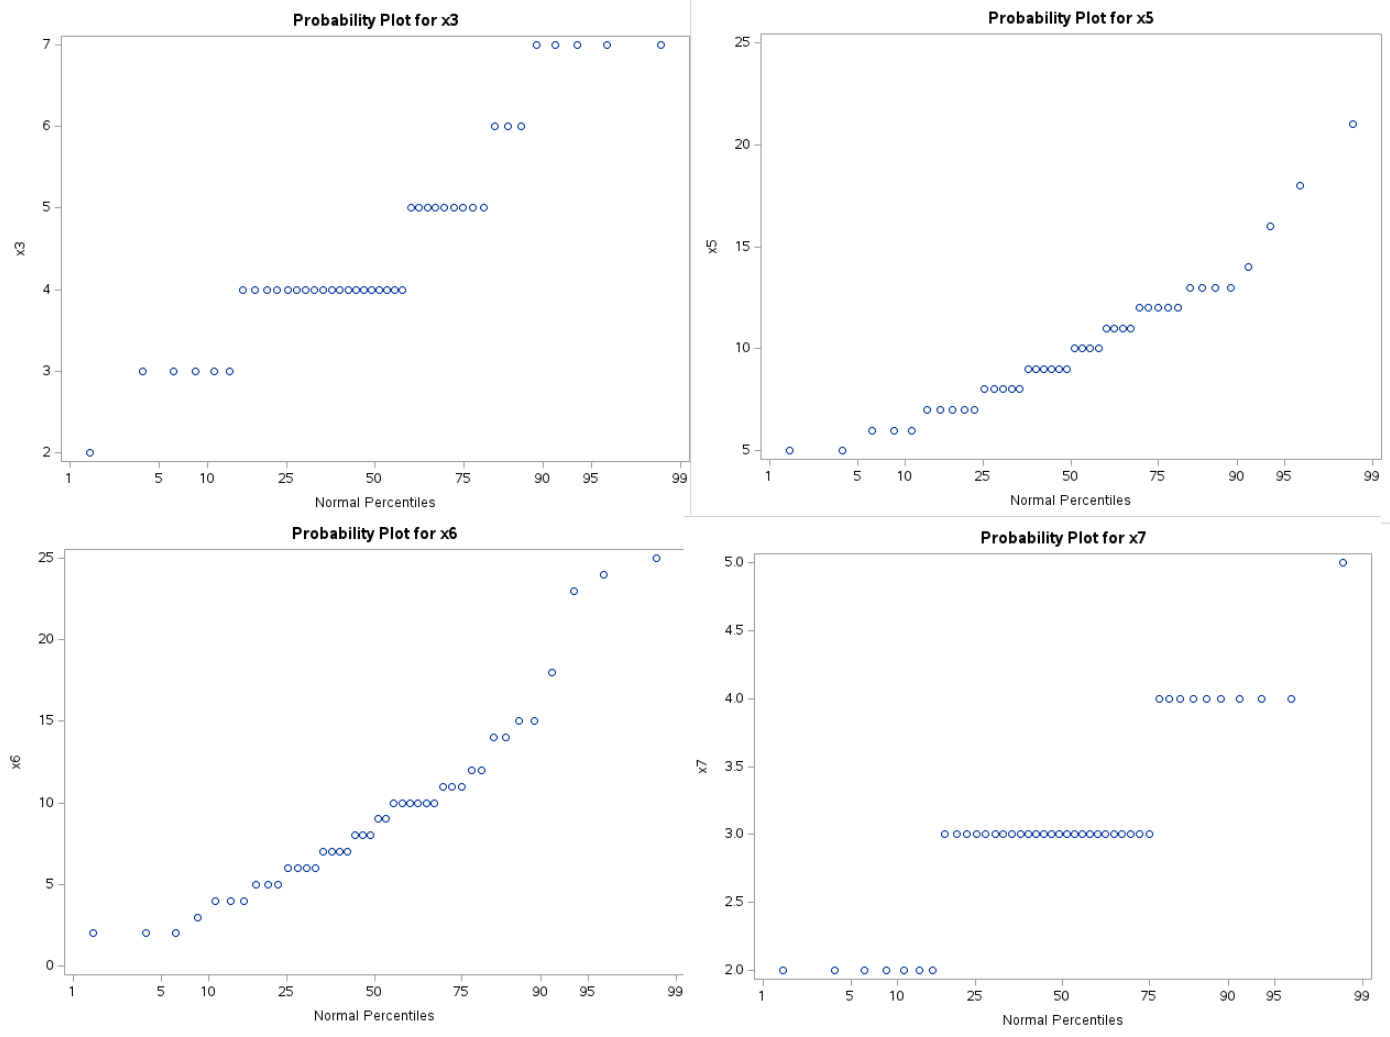
\includegraphics[width=0.6\textwidth]{Selection_1131.png} 
    \caption{SAS solution for part B.}
    \label{fig:sas1}
\end{figure}

Based on the normal probability plots seen in the Figure \ref{fig:sas1}, assumptions for normal probability are broken for CO (x3) and HC (x7), as evidenced by the deviation from the diagonal of the plot.

        \item Provide a matrix of scatterplots for the four variables above in (b). Also, report the numeric correlation for each pair of variables. Is any pair significantly correlated? Answer this with separate confidence intervals of correlation. Use a Bonferroni adjustment for multiplicity so that your confidence for all intervals simultaneously is 95\%. \\ \\

        \begin{figure}[htbp]
    \centering
    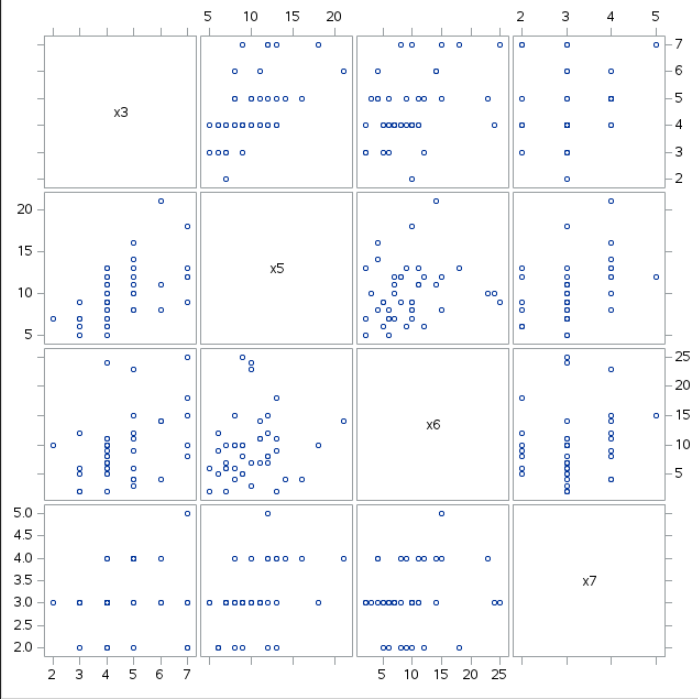
\includegraphics[width=0.6\textwidth]{Selection_1132.png} 
    \caption{SAS solution for part C. }
    \label{fig:sas2}
\end{figure}

       \begin{figure}[htbp]
    \centering
    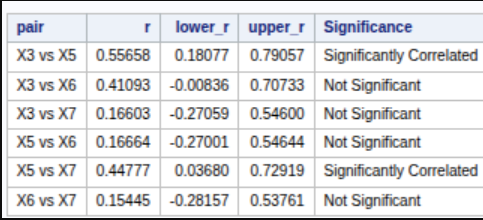
\includegraphics[width=0.6\textwidth]{Selection_1133.png} 
    \caption{SAS solution for part C with Bonferroni adjustment. }
    \label{fig:sas3}
\end{figure}

As seen in Figures \ref{fig:sas2} and \ref{fig:sas3}, only the variables that are correlated are the pair CO (x3) and NO (x5)  and the pair NO (x5) and HC (x7).
        
    \end{enumerate}

    \vspace{0.5cm}

\pagebreak

    \item \textit{(adapted from J\&W Exercise 5.7)} The variables in ``sweat.csv'' are sweat rate, sodium, and potassium for a sample of $n = 20$ females.
    
    \begin{verbatim}
    data sweat;
    infile "/sweat.csv" delimiter="," firstobs=2;
    input rate na k;
    run;
    \end{verbatim}
    
    \begin{enumerate}
        \item Find 90\% individual one-at-a-time confidence intervals for the population means of the three variables using the univariate $t$-distribution. \\ \\
        
       \begin{figure}[htbp]
    \centering
    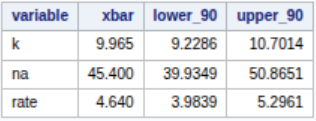
\includegraphics[width=0.6\textwidth]{Selection_1134.png} 
    \caption{SAS solution for part A. }
    \label{fig:sas4}
\end{figure}

As depicted in Figure \ref{fig:sas4}, the individual confidence intervals are (9.2286, 10.7014) for k, (39.9349, 50.8651) for na, and (3.9839, 5.2961) for rate. \\ \\
        
        \item Find 90\% ``simultaneous'' confidence intervals for the population means of the three variables (using the multiplier based on the $F$ distribution). \\ \\
        

       \begin{figure}[htbp]
    \centering
    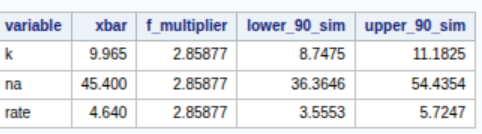
\includegraphics[width=0.6\textwidth]{Selection_1135.png} 
    \caption{SAS solution for part B. }
    \label{fig:sas5}
\end{figure}

As depicted in Figure \ref{fig:sas5}, the simultaneous confidence intervals are (8.7475, 11.1825) for k, (36.3646, 54.4354) for na, and (3.5553, 5.7247) for rate. \\ \\
        
        \item How do the interpretations of these two sets of intervals compare with one another? Why are those in (b) wider? \\ \\
        
        The multiplier in part (a) is 1.729 while the multiplier in part (b) is 2.859. The larger value in part (b) yields a larger confidence interval. \\
        
        \item The researchers were also interested in whether the population mean vector differed from $\mu_0 = [4, 50, 10]'$, and in a formal test they rejected this vector at the $\alpha = .10$ level. Is this consistent with your results in (b) above? Why or why not? \\ \\
        
		No, this is inconsistent with the findings from part (b) as the vector $[4, 50, 10]$ falls within the 90\% confidence interval for all three variables.


    \end{enumerate}
\end{enumerate}

\end{document}